\subsection{Premières \routes{} \& composants React}

\subsubsection[welcome!]{welcome!\label{sec:welcome!}}
En \laravel{} + \inertia{}, les \routes{} se trouvent toujours dans \verb|routes/web.php|.  
Une \route{}, c’est simplement un chemin que Laravel surveille. Quand quelqu’un visite ce chemin dans le navigateur, Laravel sait quoi afficher.

Voici la route par défaut que vous trouverez dans un projet neuf :
\begin{figure}[H]
    \centering
    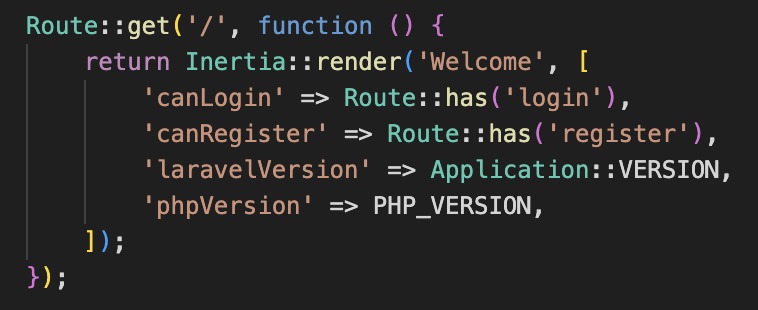
\includegraphics[width=0.75\textwidth]{figures-C1/basic_route.png}
\end{figure}

\begin{itemize}
    \item \verb|Route::get('/', ...)| signifie : « Quand quelqu’un va à l’adresse \verb|/| (la page d’accueil), fais ce qu’il y a dans les accolades ».
    \item Ici, on utilise \verb|Inertia::render('Welcome')| pour dire à Laravel : « Affiche la page React \texttt{Welcome} ».
    \item \texttt{Welcome} correspond à un fichier \verb|Welcome.jsx| qui se trouve dans \verb|resources/js/Pages|.
\end{itemize}

\subsubsection[Welcome]{Welcome}

\begin{figure}[H]
  \centering
  \begin{minipage}[t]{0.50\textwidth}
    \vspace{0pt}\raggedright
    Allons voir le fichier \verb|Welcome.jsx|. \\
    Par défaut, il contient beaucoup de code inutile pour notre formation : styles, textes et boutons de démonstration.  
    On va tout effacer et repartir d’une base simple.\\
    Voici à quoi ressemble le fichier \verb|Welcome.jsx| après nettoyage.
    Il ne contient qu’un composant React minimal, prêt à accueillir notre contenu.
  \end{minipage}\hfill
  \begin{minipage}[t]{0.40\textwidth} % réduit de 0.46 à 0.40
    \vspace{0pt}\centering
    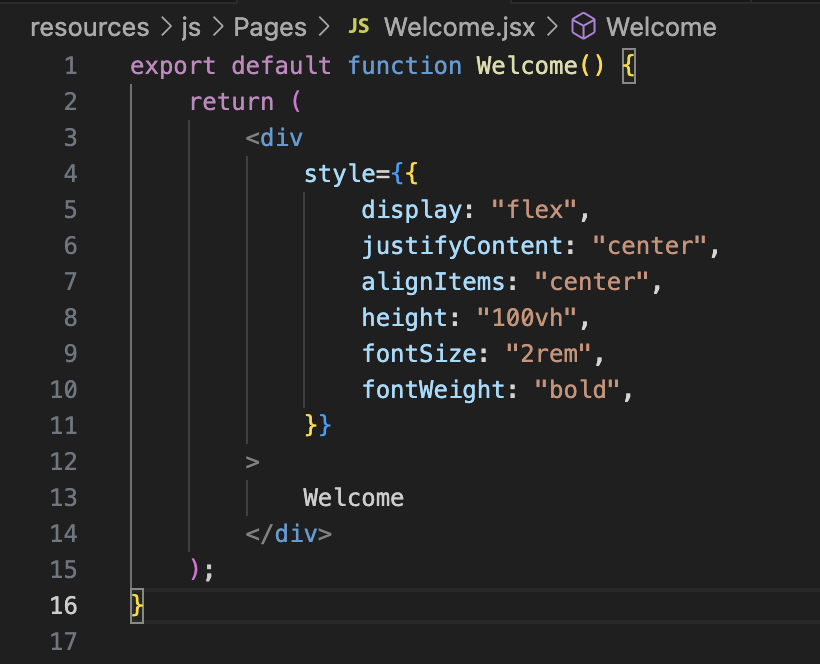
\includegraphics[width=0.9\linewidth]{figures-C1/welcome_jsx_empty.png} % 0.9 au lieu de 1.0
  \end{minipage}
\end{figure}

\paragraph{Explication du code}
\begin{itemize}
    \item \verb|export default function Welcome()| : on crée un composant React qui s’appelle \textbf{Welcome} et on l’exporte pour qu’il puisse être utilisé ailleurs.
    \item \verb|<div style={{ ... }}>| : on crée une boîte (\texttt{div}) et on lui applique du style directement en JavaScript grâce à la syntaxe \verb|{{ ... }}|.
    \item \verb|display: "flex"| : active \textbf{Flexbox}, une méthode pratique pour centrer des éléments.
    \item \verb|justifyContent: "center"| : centre le contenu horizontalement.
    \item \verb|alignItems: "center"| : centre le contenu verticalement.
    \item \verb|height: "100vh"| : la boîte prend toute la hauteur de l’écran (\texttt{vh} = \textit{viewport height}).
    \item \verb|fontSize: "2rem"| : définit la taille du texte à deux fois la taille normale.
    \item \verb|fontWeight: "bold"| : met le texte en gras.
\end{itemize}

\begin{center}
    \fbox{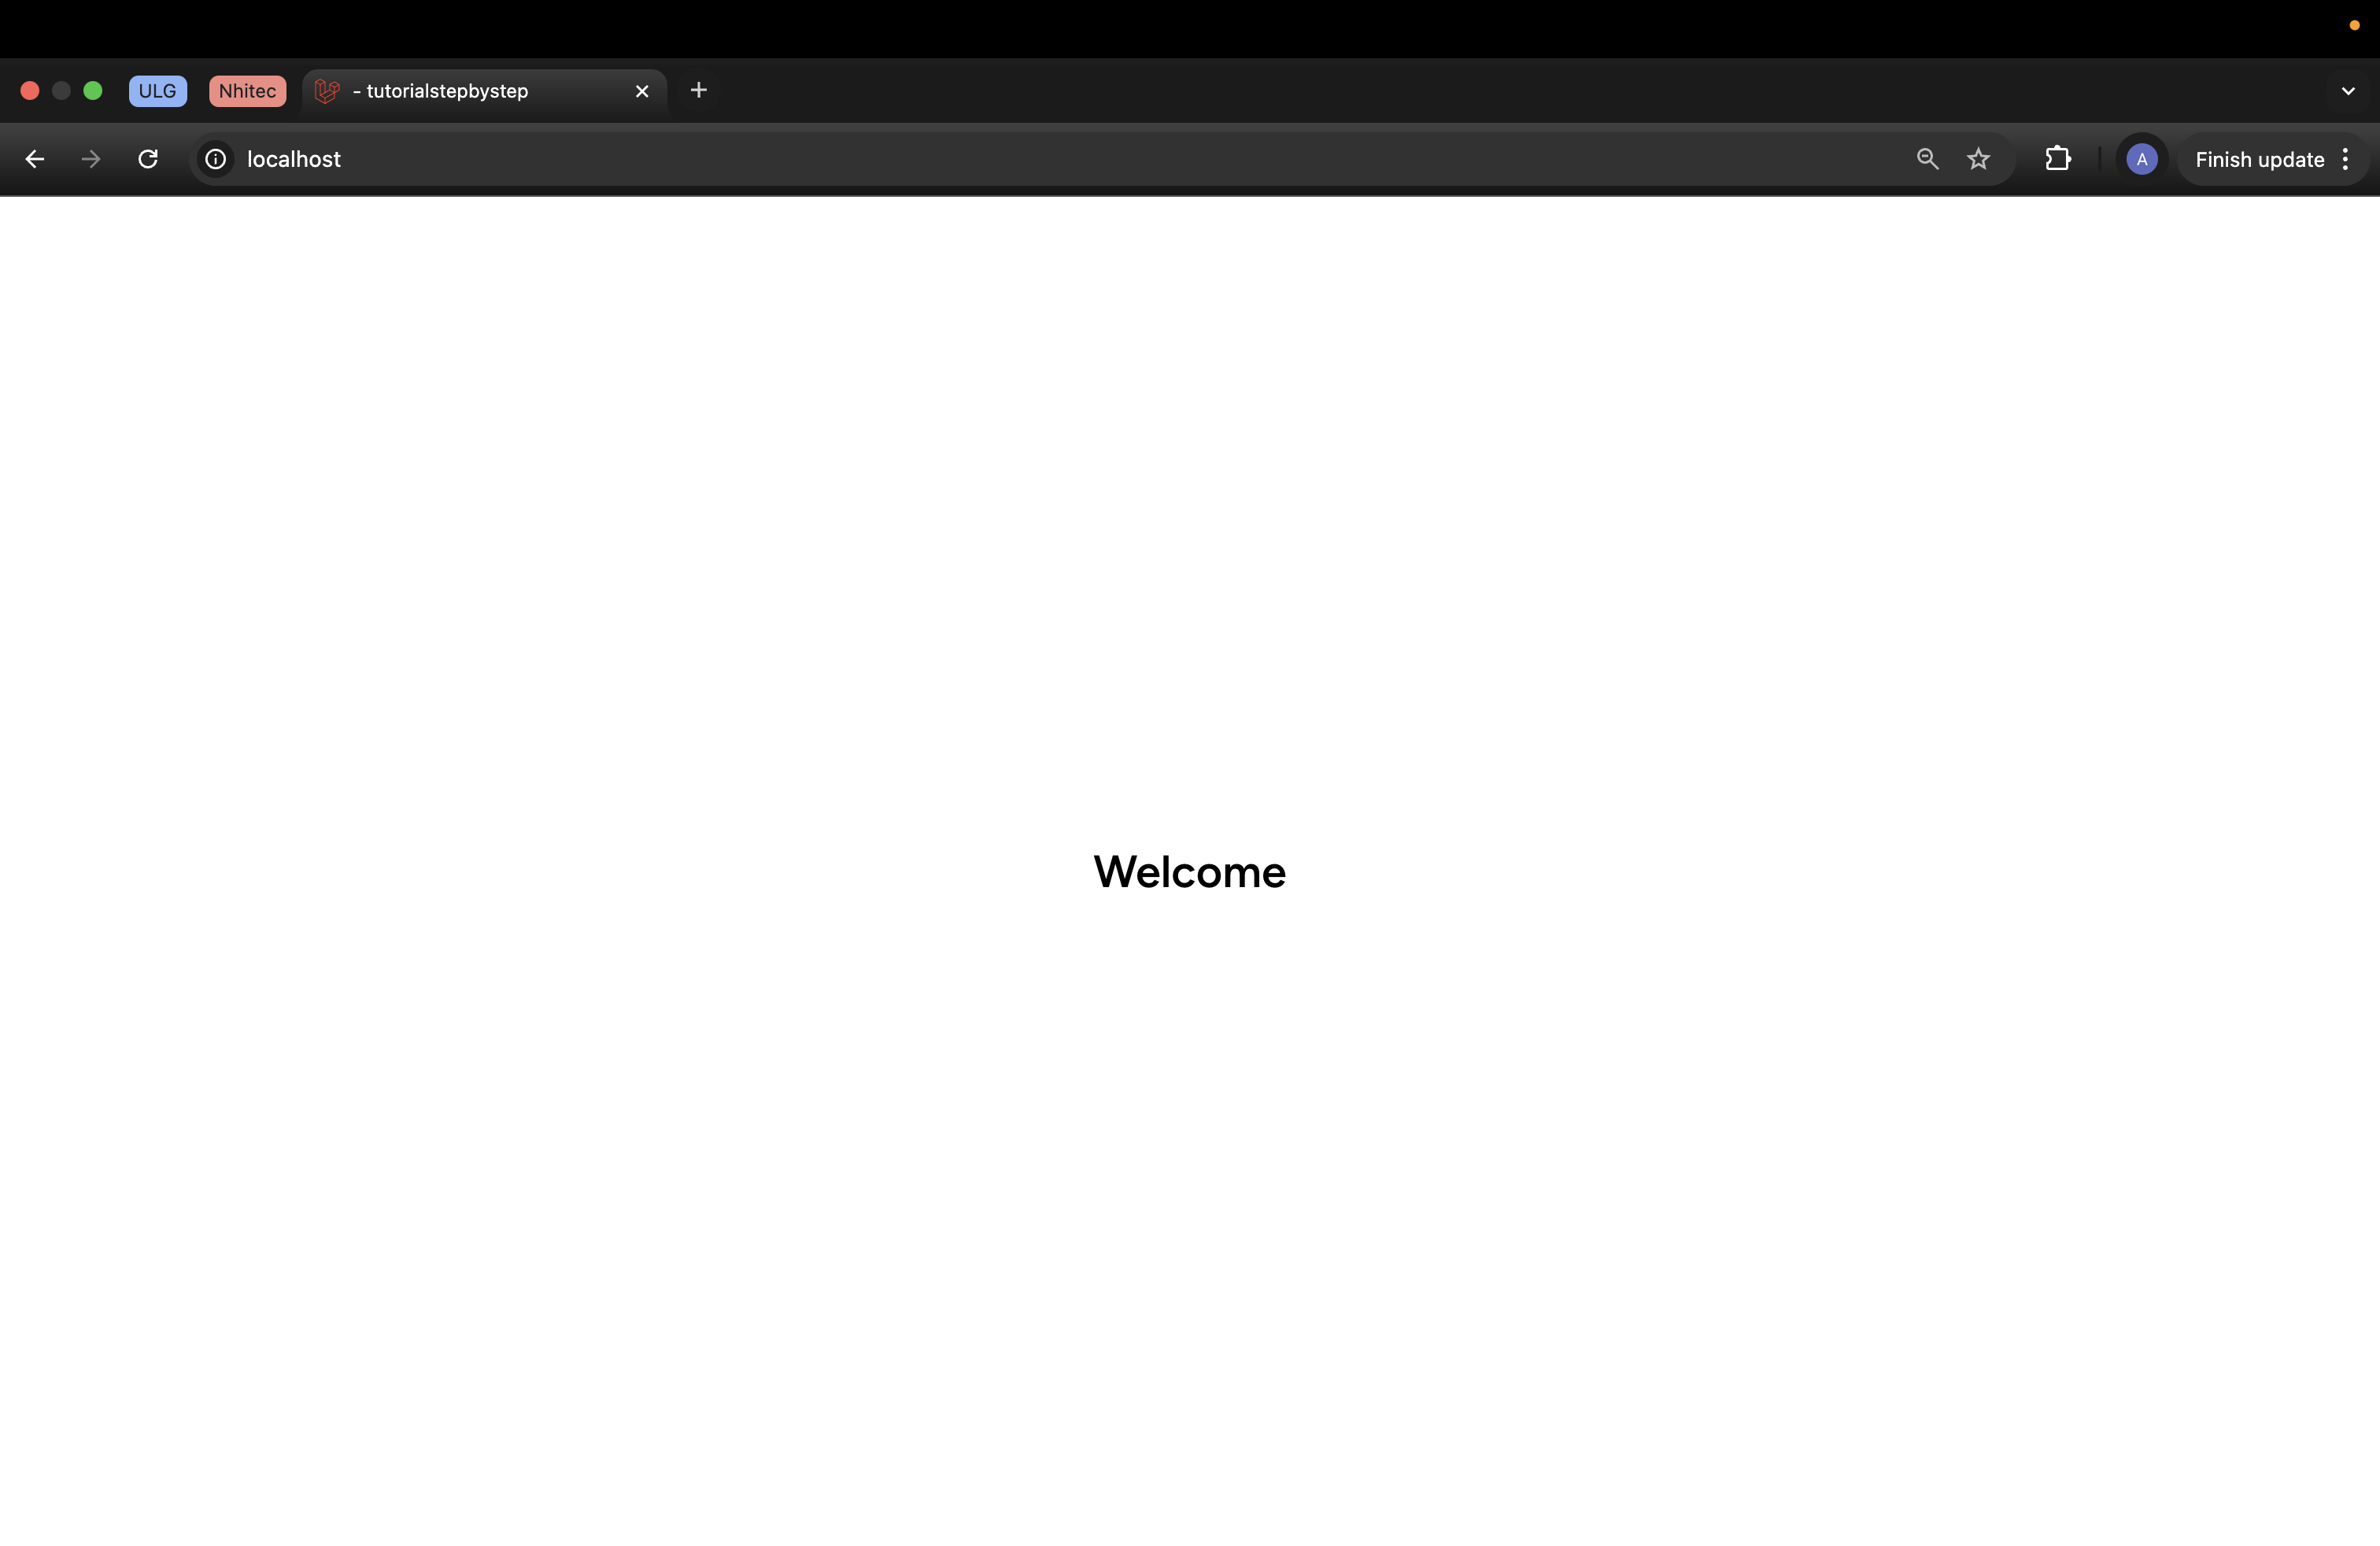
\includegraphics[width=0.65\textwidth]{figures-C1/welcome_page.png}}
\end{center}

Résultat : une page toute blanche avec juste \textbf{Welcome} bien centré, qui servira de point de départ pour construire la suite du site.

\paragraph{À retenir :}
\begin{enumerate}
    \item Les \routes{} définissent quel composant React sera affiché.
    \item \verb|Inertia::render('Welcome')| charge le fichier \verb|Welcome.jsx|.
    \item On part volontairement d’une page simple et vide pour mieux comprendre ce que l’on ajoute ensuite.
\end{enumerate}

\subsubsection[Controller][laravel.com/docs/12.x/controllers\#introduction]{Controller}

Bon, il est temps de remplir tout ça.

\begin{wrapfigure}[9]{r}{0.25\textwidth}
    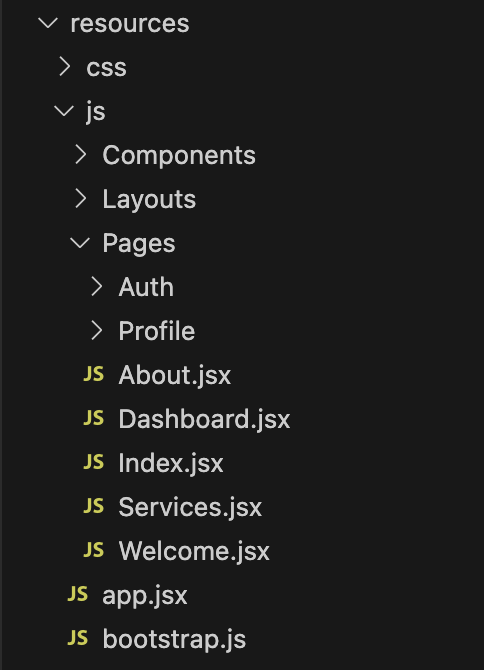
\includegraphics[width=0.25\textwidth]{figures-C1/first_views.png}
\end{wrapfigure}


On commence par préparer les pages React.  
Le dossier \verb|resources/js/Pages/| est déjà en place : ajoutez simplement trois fichiers vides \verb|Index.jsx|, \verb|Services.jsx| et \verb|About.jsx|.  
Nous y mettrons du contenu plus tard — pour l’instant ils servent juste de cibles à Inertia.

Ensuite, il nous faut un \controller{} pour relier tout ça au backend.  
Pour le créer, tapez dans le terminal :\footnote{\verb|sail artisan make:| permet de générer rapidement des fichiers (controllers, modèles, etc.).  
Comme nous utilisons \laravelsail{}, on précède \texttt{artisan} de \texttt{sail}.}

\begin{lstlisting}[language=bash]
sail artisan make:controller PagesController
\end{lstlisting}


\SaveVerb{term}|PagesController|
\begin{figure}[!h]
    \centering
    \begin{subfigure}{0.49\textwidth}
        \centering
        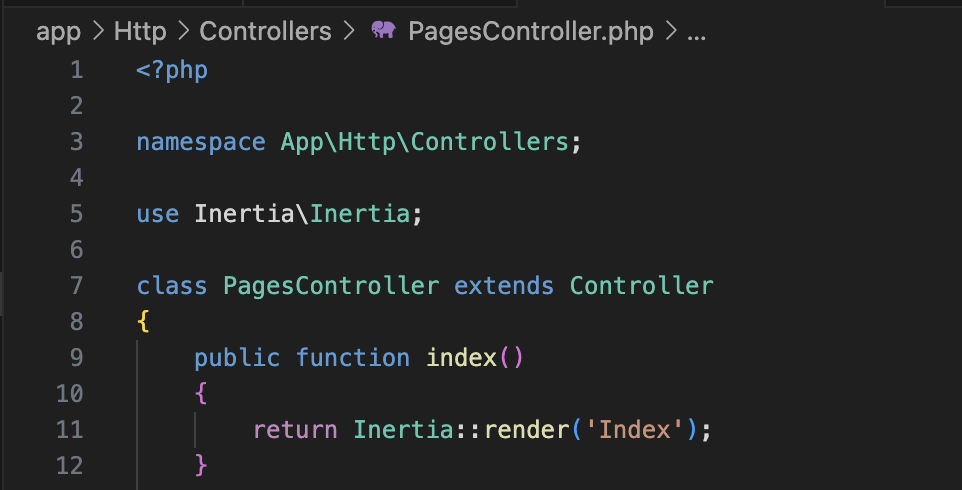
\includegraphics[width=\textwidth]{figures-C1/pages_controller_1a.png}
    \end{subfigure}
    \begin{subfigure}{0.49\textwidth}
        \centering
        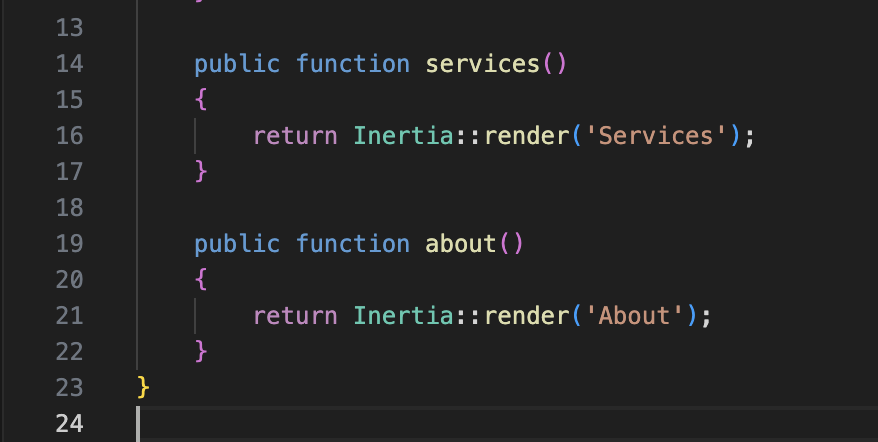
\includegraphics[width=\textwidth]{figures-C1/pages_controller_1b.png}
    \end{subfigure}
    \caption{\protect\UseVerb{term}\label{fig:PagesController1}}
\end{figure}

Le fichier généré se trouve dans \verb|app/Http/Controllers|.  
On y ajoutera trois méthodes (\verb|index|, \verb|services|, \verb|about|) qui pointeront vers nos composants React.

\newpage 

Pour avoir un premier rendu (même minimal), déposons un simple titre dans chacun des trois composants React créés plus haut.  
Cela nous permettra de vérifier que les routes affichent bien la bonne page.

\begin{figure}[H]
    \centering
    \begin{subfigure}[b]{0.31\textwidth}
        \centering
        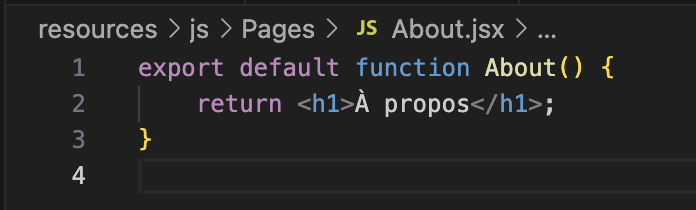
\includegraphics[width=\textwidth]{figures-C1/about_ini.png}
    \end{subfigure}
    \begin{subfigure}[b]{0.31\textwidth}
        \centering
        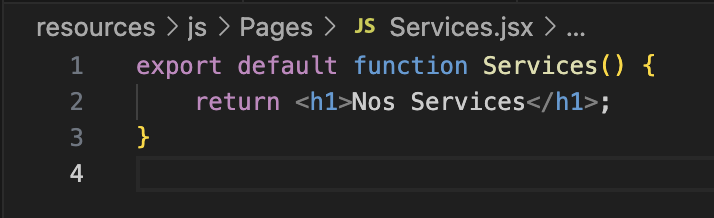
\includegraphics[width=\textwidth]{figures-C1/services_ini.png}
    \end{subfigure}
    \begin{subfigure}[b]{0.31\textwidth}
        \centering
        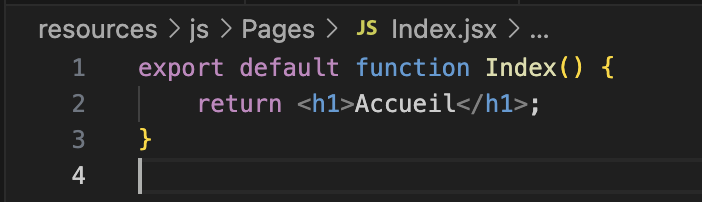
\includegraphics[width=\textwidth]{figures-C1/index_ini.png}
    \end{subfigure}
    \caption{Contenu minimal des composants React : \texttt{About} (gauche), \texttt{Services} (milieu) et \texttt{Index} (droite).}
\end{figure}

Enfin, pour pouvoir admirer le fruit de votre labeur, créez les \routes{} correspondantes dans \verb|routes/web.php|.  
On déclare notre \controller{}, puis on associe chaque URL à la bonne méthode. Résultat : aller sur \verb|/| affiche la page d’accueil, \verb|/services| la page des services, et \verb|/about| la page « À propos ».

\begin{figure}[H]
    \centering
    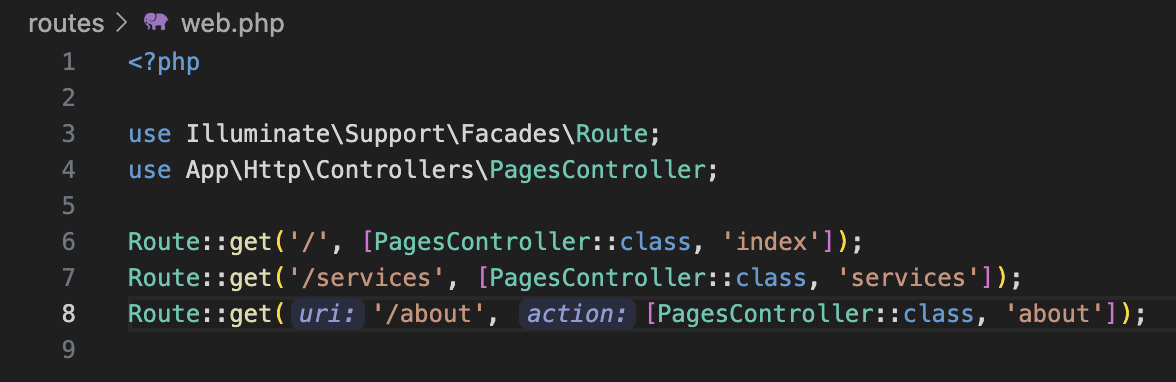
\includegraphics[width=0.7\textwidth]{figures-C1/routes_ini.png}
    \caption{}
\end{figure}

Comme toujours, le premier argument d’une route est l’adresse, et le second indique quel \controller{} et quelle méthode exécuter.  
Ici, chaque méthode retournera \verb|Inertia::render('NomDePage')|, ce qui affichera le composant React correspondant.

\begin{figure}[H]
    \centering
    \fbox{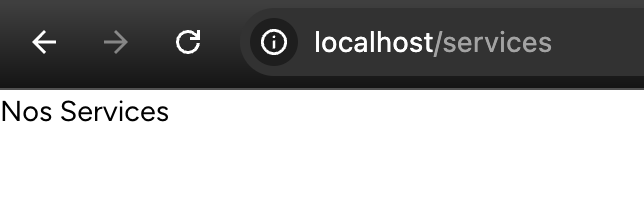
\includegraphics[width=0.55\textwidth]{figures-C1/page_services.png}}
    \caption{Affichage minimal de la page \texttt{Services} via React + Inertia.}
\end{figure}

C’est basique, pas très joli — et c’est normal. À la prochaine section, on ajoute un layout React commun et on commence à styliser l’ensemble.
